\documentclass{article}
\usepackage[margin=.75in]{geometry}
\usepackage{graphicx, dblfloatfix}
\usepackage{amsmath, amssymb, amsfonts, mathrsfs, mathtools}
\usepackage[english]{babel}
\usepackage[autostyle, english = american]{csquotes}
\usepackage[normalem]{ulem}
\usepackage[title,titletoc,toc]{appendix}
\MakeOuterQuote{"}

\newcommand{\redchi}{$\tilde{\chi}^2\,$}
\DeclareMathOperator{\erf}{erf}
\DeclareMathOperator{\cov}{cov}
\newcommand{\diverg}[1]{\ensuremath{\vec{\nabla} \cdot {#1}}}
\newcommand{\curl}[1]{\ensuremath{\vec{\nabla} \times {#1}}}
\newcommand{\dipole}{$\vec{\mu}\,$}
\newcommand{\B}{$\vec{B}\,$}
\newcommand{\E}{$\vec{E}\,$}
\DeclarePairedDelimiter\abs{\lvert}{\rvert}%
\DeclarePairedDelimiter{\parens}{\lparen}{\rparen}

\title{Electron Spin Resonance}
\author{Aman LaChapelle}

\begin{document}
\raggedright
\maketitle

\begin{abstract}
	The classical example of a magnetic dipole moment reacting in a magnetic field is the electron.  Here we will investigate the reaction of a particle with a dipole moment in a magnetic field and investigate how it changes in analogy to the electron.  We begin with a classical analogue of the electron and move on to an ensemble of electrons.  These electrons are bound in DPPH, rather than being a 3D gas, but for all intents and purposes will serve to illustrate the properties we are investigating here.
\end{abstract}

\tableofcontents
\newpage

\section{Introduction}
	The magnetic dipole moment of a charged particle is related to the spin of the particle in the simple analogue of a current loop.  Charges going around a closed loop have a magnetic dipole moment
	\begin{equation*}
		\vec{\mu} = IA\hat{n}
	\end{equation*}
	with $\hat{n}$ being the unit vector normal to the area $A$.  This generates a magnetic dipole field, equal to
	\begin{equation*}
		B = \frac{\mu_0}{4\pi}\bigg{(}\frac{3r(\vec{\mu} \cdot \vec{r})}{r^5} - \frac{\mu}{r^3}\bigg{)}.
	\end{equation*}

	This assumes no external field, however.  If there is an external field, and \dipole is not perfectly aligned, we will see precession about the external field (assuming a DC field pointing in one direction).  We can measure this property both in our classical analogue to an electron, and in actual electrons.  This effect is also very important in other areas of physics.  For example, in microwave resonators we use crystals of Yttrium-Iron-Garnet which have the property that an AC \B field of approximately 2000 Gauss will cause them to precess at microwave frequency in such a way that couples strongly to the resonator.  This has many useful applications, and there is some extremely interesting physics we can study simply by looking at the precession of the magnetic dipole moment.



\section{Theory}
	\subsection{Classical System}
	We can derive the precession about the external field beginning with the torque felt by \dipole when placed in an external field.  We will begin with the Maxwell Stress Tensor.  In the case of a dipole moment that is not aligned to the external field, we see that the stress tensor is asymmetric.  Since the stress tensor is given (in this case - neglecting the small \E fields) by
	\begin{equation*}
		\sigma_{ij} = \frac{H_iH_j}{4\pi} - \frac{H^2}{8\pi}\delta_{ij}
	\end{equation*}
	for situations in vacuum.  We realize from this equation that if two fields are not colinear then the tensor will be asymmetric.  In order to recover the symmetry (and minimize the energy by aligning the fields), there will be some torque on the object.  Furthermore, since we are interested in the magnetic dipole moment let us recognize that
	\begin{equation*}
		H = \frac{B}{\mu_0} - \int_{V}\vec{\mu}\,dV.
	\end{equation*}
	Thus we can write
	\begin{gather*}
		\tau_i = -\epsilon_{ijk}\sigma_{jk}\\
		\tau_i = -\epsilon_{ijk}\frac{H_jB_k}{4\pi}\\
		\vec{\tau} = \frac{-\vec{H} \times \vec{B}}{4\pi}
	\end{gather*}
	\begin{equation}
		\vec{\tau} = \vec{\mu} \times \vec{B}
	\end{equation}
	with $\epsilon_{ijk}$ being the Levi-Cevita tensor and the subscripts denoting components of the respective object.

	\vspace{.25cm}

	Now that we know the torque exerted on the magnetic moment by the external field, we can begin to work through the precession and the frequency of precession caused by that torque.
	\vspace{.25cm}

	\begin{figure}[!htb]
		\centering
		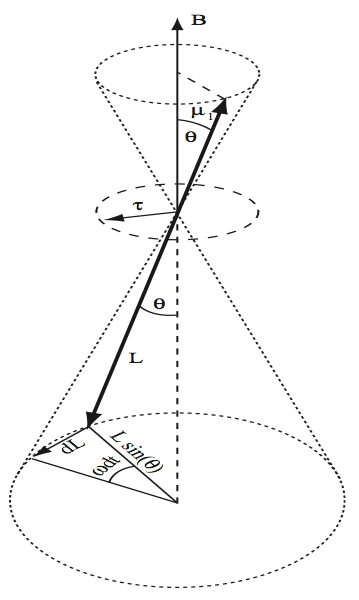
\includegraphics[scale=.5]{../figures/torque}
		\caption{The precession of \dipole about an external \B field.}
	\end{figure}

	Figure 1 provides us with some intuition into how to go about finding the frequency of precession of the dipole moment.  Since we can transform into a rotating frame to describe the motion of $\vec{L}$, we can write
	\begin{gather*}
		\frac{d\vec{L}}{dt} = \vec{\tau} = \vec{\omega} \times \vec{L}\\
		\vec{\mu} \times \vec{B} = \vec{\omega} \times \vec{L}
	\end{gather*}
	and since the angle between \dipole and \B is the same as the angle between $\vec{\omega}$ and $\vec{L}$ by definition of our frame, we can write 
	\begin{gather}
		\omega = \frac{\mu}{L}B\\
		\omega = \gamma B
	\end{gather}
	where $\gamma$ is the gyromagnetic ratio of the object in question.

	\subsection{Quantum System}
	We can express the quantum system and its energy using a simple Hamiltonian.  Since we have an electron precessing in a \B field, we know that $\mathscr{H}$ will be given by
	\begin{gather*}
		\mathscr{H} = \frac{\hat{p}^2}{2m} \nabla^2 + V\\
		\hat{p} = -i\hbar \nabla \rightarrow \hat{p}_{\tiny{e\!f\!f}} = -i\hbar \nabla + \frac{e}{c}A\\
		V = -e\phi\\
	\end{gather*}
	so we can write $\mathscr{H}$ as
	\begin{equation}
		\mathscr{H} = -\frac{\hbar^2}{2m} \nabla^2 -\frac{ie\hbar}{2mc} \big{(}\vec{\nabla}\cdot\vec{A}\big{)} - \frac{ie\hbar}{mc}\big{(}\vec{A}\cdot\vec{\nabla}\big{)} + \frac{e^2}{2mc^2}A^2 - e\phi.
	\end{equation}

	Most often this will be simplified by working in the Coulomb gauge, 
	\begin{equation*}
		\diverg{\vec{A}(\vec{r},t)} = 0
	\end{equation*}
	or the Lorenz gauge,
	\begin{equation*}
		\diverg{\vec{A}} + \frac{1}{c^2}\frac{\partial \phi}{\partial t} = 0.
	\end{equation*}

	In any case, the algebra is trivial yet lengthy and so will be left as an exercise to the reader should they wish.

	\vspace{.25cm}

	Returning to the task at hand, we can define (or derive from the above Hamiltonian, in the first perturbative expansion) the energy of a dipole moment due to an external magnetic field given by
	\begin{equation*}
		E^{(1)} = -\vec{\mu} \cdot \vec{B}
	\end{equation*}
	and so the energy splitting that acts on the free electron will be
	\begin{equation*}
		\Delta E = g_s\mu_B B
	\end{equation*}
	Where $\mu_B$ is the Bohr Magneton, $g_s$ is the dimensionless magnetic moment, and $\Delta E$ is the energy difference between the spin up and spin down states.  Thus if we inject photons with energy $\hbar \omega = \Delta E$ into the system we will be able to force the electron to change spin states.  Since our goal is to measure the gyromagnetic ratio of the electron, we will rewrite the energy shift as follows
	\begin{gather*}
		\hbar \omega = g_s\mu_B B\\
		\omega = \frac{g_s \mu_B}{\hbar} B\\
		\omega = \gamma_e B
	\end{gather*}
	where $\gamma_e$ is the gyromagnetic ratio of the electron. 

	\vspace{.25cm}

	$g_s$ is a dimensionless quantity that is predicted by the Dirac equation to be exactly 2.  However, full quantum electrodynamics introduces small corrections to $g_s$ that can be expressed as
	\begin{equation*}
		g_s = 2\bigg{(}1+\frac{\alpha}{2\pi} + ...\bigg{)}.
	\end{equation*}
	To first order, $g_s = 2$, however.




\section{Apparatus}
	\subsection{Classical System}
	For the classical system the apparatus is shown in figure 2.

	\vspace{.25cm}

	\begin{figure}[!htb]
		\centering
		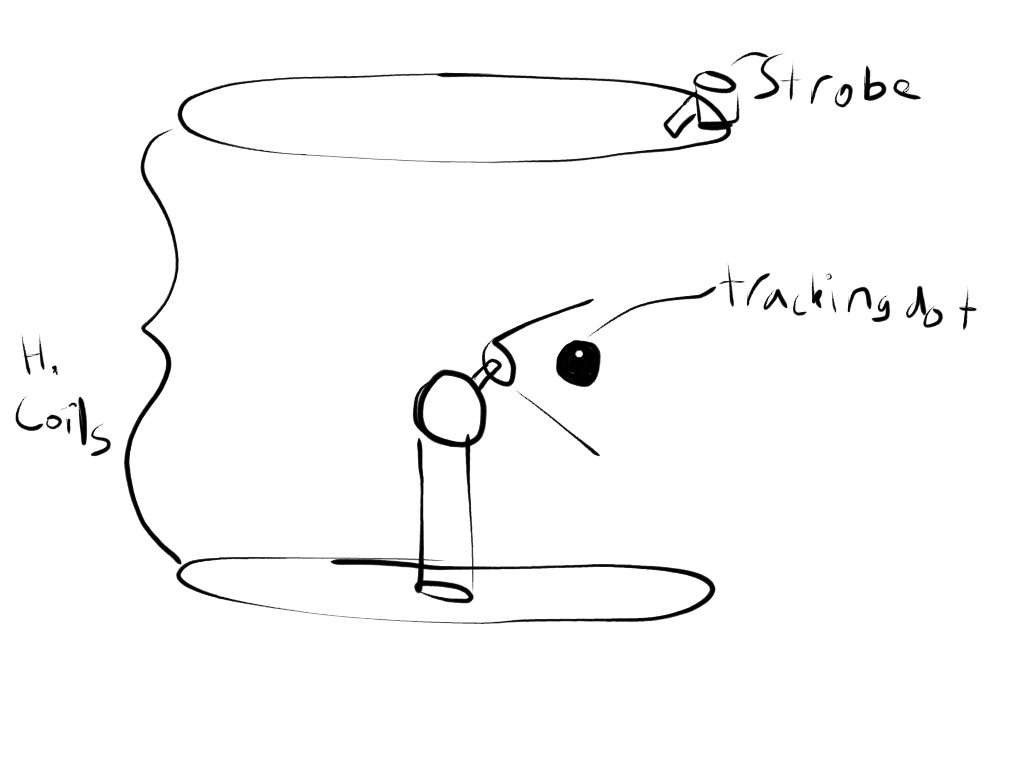
\includegraphics[scale=.35]{bigcoils.jpg}
		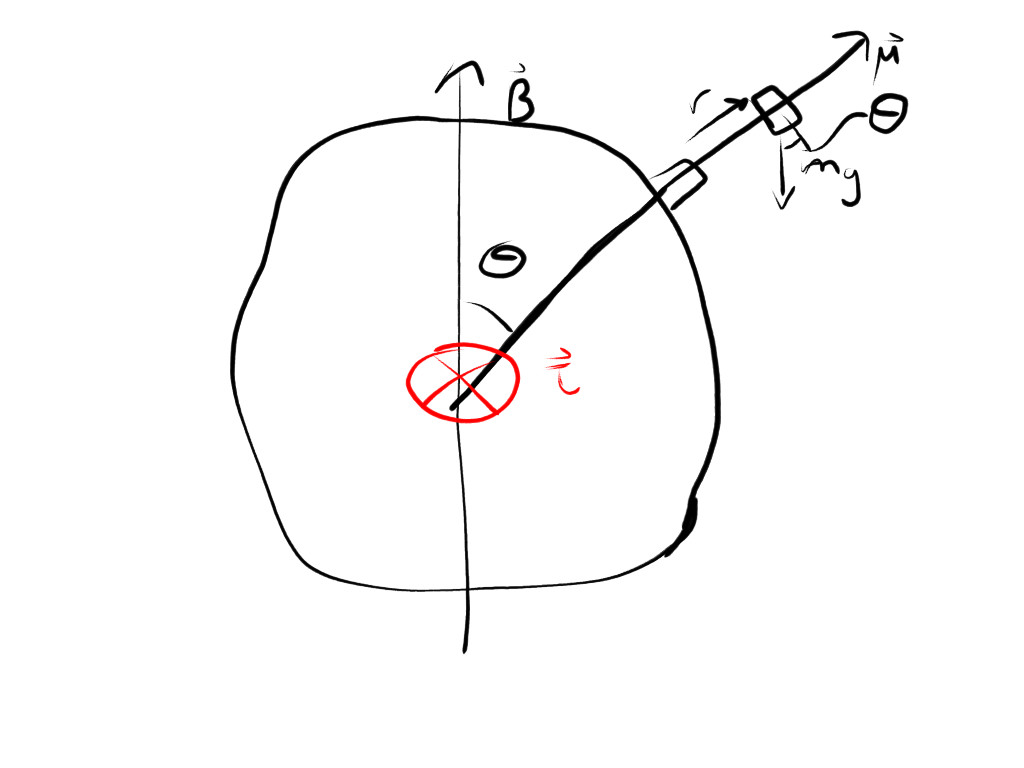
\includegraphics[scale=.35]{ball.jpg}
		\caption{The classical experiment apparatus.  Above is the macroscopic apparatus, below is the ball with the forces drawn on.  The angles are the same by virtue of the way we choose our axes.}
	\end{figure}

	We have a billiard ball with an embedded magnet whose moment is aligned along the axis of the small black handle used to spin the ball.  The ball rests on an air mount that simulates a frictionless surface and is centered between two Helmholtz coils that can be controlled to act in parallel or in opposition.  If they act in parallel we can use the relation
	\begin{equation*}
		B = I \times \bigg{(}1.36 \pm 0.003 \hspace{.1cm} \frac{T}{A}\bigg{)}
	\end{equation*}
	to convert from the value of current that the apparatus outputs to the value of \B we want.

	\vspace{.25cm}

	In order to actually take data we make use of a strobe light mounted to the Helmholtz coils to track a white dot on the ball's handle as it precesses around the external field.  We also make use of a moveable index to track the ball to measure the period of precession.  While measuring the magnetic moment via the gravitational torque, we use a aluminum rod with a steel end that has a sliding mass mounted to it.  This serves as a means to adjust the torque on the ball due to gravity so that we can measure what \B is required to balance the gravitational force.

	While working through the spin flip portion, we used a saddle that contains fixed permanent magnets to create a \B field perpendicular to the Helmholtz coils.  Spinning this saddle at the correct frequency will create the spin flip phenomenon observed.

	\subsection{Quantum System}
	For the quantum system the apparatus is shown in figure 3.

	\vspace{.25cm}

	\begin{figure}[!htb]
		\centering
		\includegraphics[scale=.5]{esr_connections.png}
		\caption{Basics of the ESR apparatus.}
	\end{figure}

	We use the Deadalon ESR apparatus, consisting of a 60 Hz AC power supply for the large Helmholtz coils, a tunable RF oscillator, and Helmholtz coils connected such that \B at the center will be given by
	\begin{equation*}
		B = I \times \bigg{(}0.48 \hspace{.1cm} \frac{mT}{A}\bigg{)}.
	\end{equation*}
	$I$ is the sum of currents flowing in each coil.  At the center of both the large Helmholtz coils and the RF oscillator is a sample probe containing a small amount of DPPH, a substance containing stable free radicals that allow measurement of the Electron Spin Resonance.  DPPH is a polymer that contains about 1 free spin per 41 atoms.  It is typically paramagnetic, which means that it has unpaired spins that are random and free to be aligned rather than having some sort of alignment predetermined.  DPPH is a common standard for the measurement of Electron Paramagnetic Resonance (Electron Spin Resonance) and is well documented for this use.

	\vspace{.25cm}

	DPPH is typically calibrated so it has a $g_s$ of approximately 2.0036. \cite{DPPH}  Since $g_s$ is so close to what we would see in a free electron, and since DPPH is stable in a configuration that has this free spin (free electron, as far as our purposes require) it will allow us to model the behavior of the free electron to a not inaccurate approximation.  Thus any uncertainty introduced is purely from the data taking procedure and the inherent inaccuracy of aligning a line on a digital display.

	\vspace{.25cm}

	Incidentally, the images seen on the oscilloscope are reproduced in figure 4.

	\begin{figure}[!htb]
		\centering
		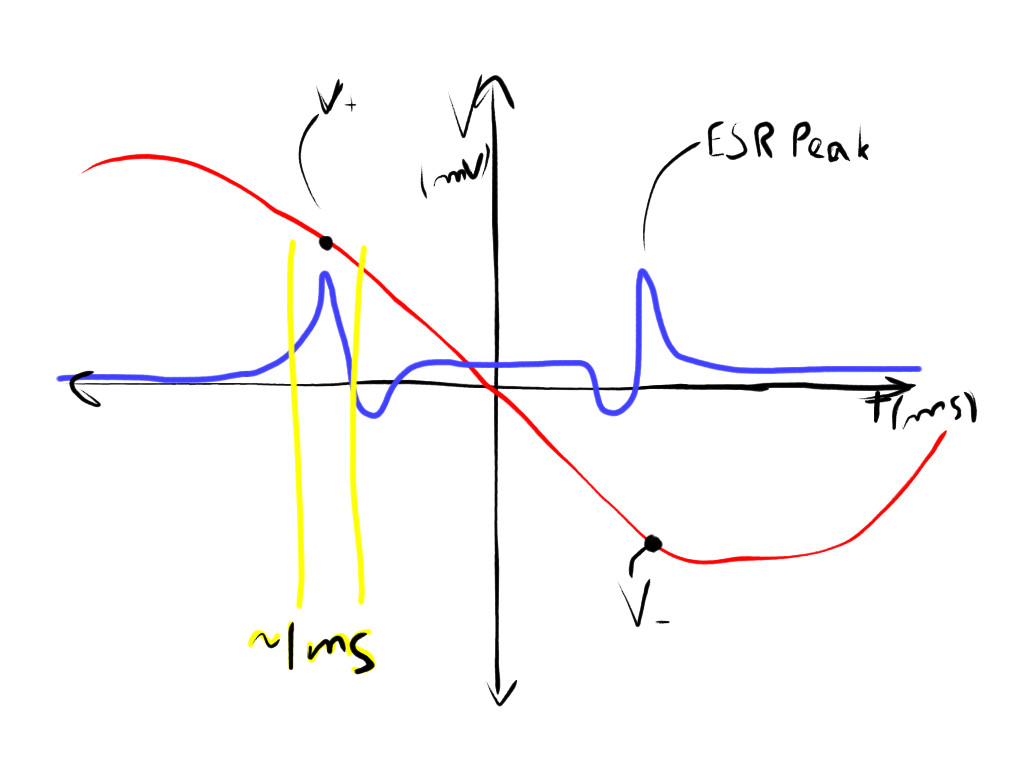
\includegraphics[scale=.35]{esrpeaks.jpg}
		\caption{A rendering of the Oscilloscope view.}
	\end{figure}




\section{Data Analysis}
	Note: All plots in this section use the notation $Ae\!+\!b$ to mean $A \times 10^{b}$.  Not meant to cause confusion, simply due to quirks with formatting in the Python language.
	\subsection{Gravitational Torque Balancing}
	We measured the magnetic dipole moment of the ball by measuring the torque on the ball due to gravity, calculated by measuring the sliding mass mentioned earlier.  A figure is most illustrative of the results, with data tabulated below.

	\begin{figure}[!htb]
		\centering
		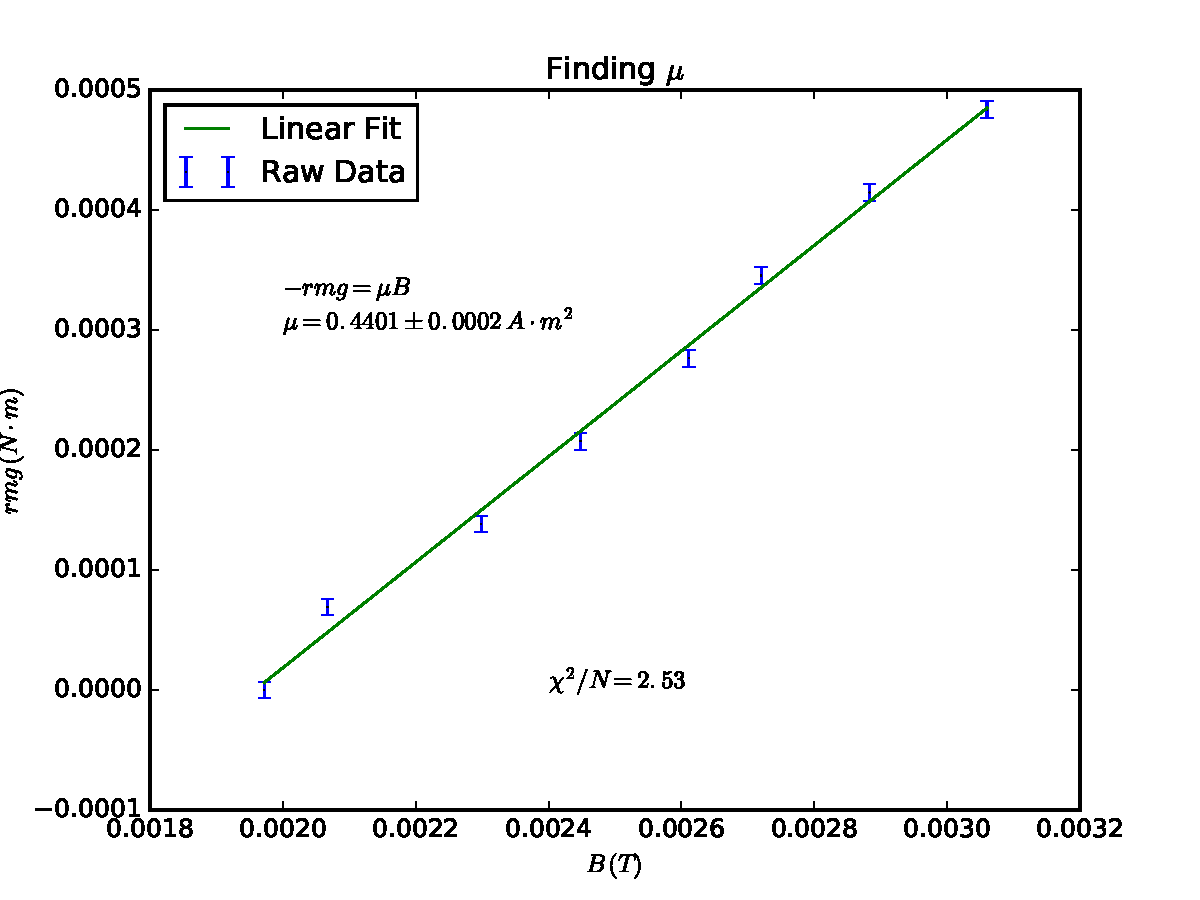
\includegraphics[scale=.5]{../plots/rmgvsmub.pdf}
		\caption{Shown is a plot of the gravitational torque vs the torque due to the magnetic dipole moment.  The fit has a \redchi of 2.53, mainly due to the small error in the experiment, possibly underestimated, as we did not take into account friction on the ball in its mount.}
	\end{figure}

	\begin{center}
	\begin{tabular}{|l|l|}
		\hline
		$\vec{B} \pm \delta\vec{B} \, (T)$ & $rmg \pm \delta rmg \, (N \cdot m)$ \\
		\hline
		$(1.9 \pm 0.4) \times 10^{-3}$ & $(0 \pm 0.7) \times 10^{-5}$ \\
		$(2.1 \pm 0.4) \times 10^{-3}$ & $(6.9 \pm 0.7) \times 10^{-5}$ \\
		$(2.3 \pm 0.5) \times 10^{-3}$ & $(1.38 \pm 0.07) \times 10^{-4}$ \\
		$(2.4 \pm 0.5) \times 10^{-3}$ & $(2.07 \pm 0.07) \times 10^{-4}$ \\
		$(2.6 \pm 0.5) \times 10^{-3}$ & $(2.76 \pm 0.07) \times 10^{-4}$ \\
		$(2.7 \pm 0.5) \times 10^{-3}$ & $(3.45 \pm 0.07) \times 10^{-4}$ \\
		$(2.9 \pm 0.5) \times 10^{-3}$ & $(4.14 \pm 0.07) \times 10^{-4}$ \\
		$(3.1 \pm 0.6) \times 10^{-3}$ & $(4.84 \pm 0.07) \times 10^{-4}$ \\
		\hline
	\end{tabular}
	\end{center}

	We should note that these uncertainties are calculated by
	\begin{gather*}
		\delta B = \sqrt{ \parens*{\frac{.002}{1.36}}^2 + \parens*{\frac{\delta I}{I}}^2 } \times B\\
		\delta (rmg) = \sqrt{ \parens*{\frac{\delta r}{r}}^2 + \parens*{\frac{\delta m}{m}}^2 } \times (rmg)
	\end{gather*}

	\vspace{.25cm}

	This gives a value of $\mu$,

	$$\boxed{\mu = 0.4401 \pm 0.0002 \, A \cdot m^2}$$

	Since we have nothing to compare this value to, we will continue, for the moment, to our measurement of the gyromagnetic ratio and associated magnetic dipole moment in order to compare the two values and speak quantitatively about the experiment and our uncertainties.

	\subsection{Precession of \sout{a Billiard Ball} an Electron}
	In this section we added angular momentum to the ball, and then used the strobe light to time its rotation frequency (its spin).  Once we knew the spin of the ball, we then turned on the external \B field and timed its precession using the moveable index.  Again, a graph is most illustrative and will serve to show our values best, data values tabulated below.

	\begin{figure}[!htb]
		\centering
		\includegraphics[scale=.5]{../plots/omegavsb.pdf}
		\caption{The observant reader will notice that this measurement has a \redchi of 0.210, which is very low.  This is due, again, to the error in the experiment, and the imprecise nature of using a stopwatch on strobe-fatigued eyes.}
	\end{figure}

	\begin{center}
	\begin{tabular}{|l|l|}
		\hline
		$\omega \pm \delta \omega \, (H\!z)$ & $\vec{B} \pm \delta \vec{B} \, (T)$ \\
		\hline
		$(4.71 \pm 0.12) \times 10^{-1}$ & $(1.2 \pm 0.2) \times 10^{-3}$ \\
		$(5.5 \pm 0.3) \times 10^{-1}$   & $(1.4 \pm 0.3) \times 10^{-3}$ \\
		$(7.9 \pm 0.5) \times 10^{-1}$   & $(2.0 \pm 0.4) \times 10^{-3}$ \\
		$1.15 \pm 0.07$ 			     & $(2.7 \pm 0.5) \times 10^{-3}$ \\
		$1.39 \pm 0.08$ 			     & $(3.4 \pm 0.7) \times 10^{-3}$ \\
		$1.7 \pm 0.1$ 				     & $(4.1 \pm 0.8) \times 10^{-3}$ \\
		\hline
	\end{tabular}
	\end{center}

	The uncertainties in $\omega$ are measured directly from the strobe output, and the uncertainties in \B are calculated the way they are above, 
	\begin{equation*}
		\delta B = \sqrt{ \parens*{\frac{.002}{1.36}}^2 + \parens*{\frac{\delta I}{I}}^2 } \times B.
	\end{equation*}
	
	\vspace{.25cm}

	This gives us values for $\mu$ and $\gamma$,

	$$\boxed{\mu = 0.47 \pm 0.04 \, A \cdot m^2}$$
	$$\boxed{\gamma = 410 \pm 14 \, Hz/T}$$

	We should note that this value of $\gamma$ has units of $\frac{rad\cdot H\!z}{T}$.

	\vspace{.25cm}

	We see agreement between our values of $\mu$ to a 0.862 $\sigma$ difference, or a confidence level of 38.87\%.  Considering the fact that the values were both calculated with quite imprecise methods leads us to the conclusion that this is an acceptable confidence level, and we will proceed as such.

	\vspace{.25cm}

	However, we also have a calculated value of $\gamma$ that we can use if we want to compare measurements.  We calculate this taking our values for the mass and radius of the ball and dividing our measured $\mu$ from the gravitational torque balancing by this value for the angular momentum.  Below we will tabulate our values (with uncertainty) for measured quantities such as the mass and radius of the ball and perform the calculation itself.

	\begin{center}
	\begin{tabular}{|l|}
		\hline
		$M \pm \delta M = 0.13738 \pm 0.00001 \, kg$ \\ \hline
		$R \pm \delta R = (2.69 \pm .05)\times 10^{-2} \, m$ \\ \hline
		$\Omega \pm \delta \Omega = 2\pi \cdot \parens{4.6 \pm 0.1} \, H\!z \, \big{(}\frac{rad}{s}\big{)}$ \\ \hline
	\end{tabular}
	\end{center}

	\begin{gather*}
		\vec{L} = \frac{2}{5}MR^2\vec{\Omega}\\
		\boxed{\vec{L} = 1.15\times10^{-3}}\\
		\delta \vec{L} = \sqrt{ \parens*{\frac{\partial L}{\partial M}\delta M}^2 + \parens*{\frac{\partial L}{\partial R}\delta R}^2 + \parens*{\frac{\partial L}{\partial \Omega} \delta \Omega}^2 }\\
		\boxed{\delta \vec{L} = 0.05\times10^{-3}}\\
		\boxed{\vec{L}\pm\delta\vec{L} = \parens*{1.15 \pm 0.05}\times10^{-3} \, \, \frac{kg \, m^2}{s}}.
	\end{gather*}
	And so if we take this value for $L$ and calculate $\gamma$, we get
	\begin{gather*}
		\gamma = \frac{\mu}{L}\\
		\mu = 0.4401 \pm .0002 \, A\cdot m^2\\
		\delta\gamma = \sqrt{ \parens*{\mu \cdot \delta L}^2 + \parens*{\frac{1}{L}\cdot\delta\mu}^2 }\\
		\boxed{\gamma \pm \delta\gamma = 382.94 \pm 0.17 \,\, \frac{H\!z}{T}}
	\end{gather*}
	since we are in SI units, with Hz being rad/sec.  If we calculate the agreement between this $\gamma$ and the $\gamma$ obtained from the fit, we see that the agree to within 1.93 $\sigma$, which gives us a confidence level of 5.36\%.  This is rather low, and so we should work on tracking down possible causes.  

	\vspace{.25cm}

	A higher confidence level would require that either the fitted $\gamma = \gamma_f$ is lower, or the calculated $\gamma = \gamma_c$ is higher.  Based on the fact that we calculated $\mu$ from the fit, and the values of $\mu$ agreed to better than 38.87\% and the uncertainty in $\mu = 0.4401 \pm 0.0002$ is much lower, we believe the more likely cause is the high value of $\gamma_f$.  This would imply that we overestimated $\omega$ or underestimated \B.  Since our uncertainty in $\omega$ is much higher, it is more likely that we overestimated $\omega$.  If we were able to take the data again, we would focus on taking many data points at each stage of the precession to determine if our overestimation is systematic or random uncertainty.  However, because we did not have time to retake data points, we will have to live with our agreement between $\gamma_c$ and $\gamma_f$ of 5.36\%.

	\subsection{Classical Spin Flip}
	This section of the experiment deals with rotations within rotations.  In order to simplify the picture a bit, we will transform into the frame of the saddle and look at the ball from that frame.

	\begin{figure}[!htb]
		\centering
		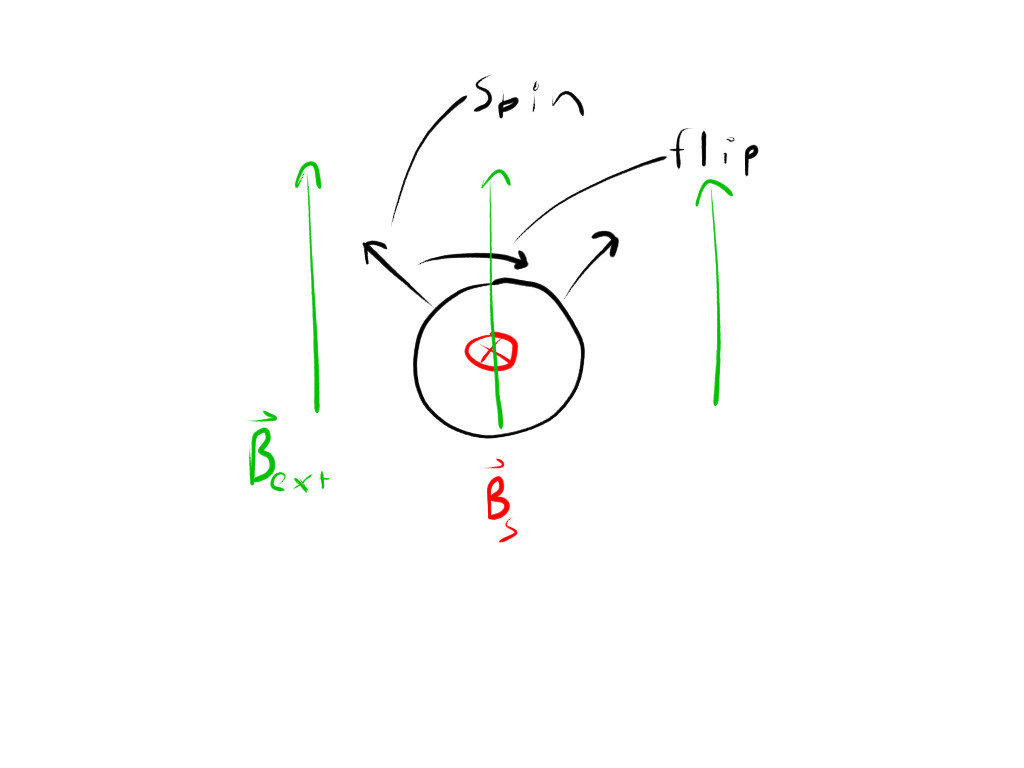
\includegraphics[scale=.5]{flip.jpg}
		\caption{A rendering of the \B fields in the frame of the saddle so as to not have to draw that rotation as well.}
	\end{figure}

	If we set the billiard ball spinning and then turn on the field, it precesses with some frequency about the external \B field.  If we rotate the saddle and its accompanying \B field with approximately the frequency of precession but in the opposite direction, we observe that the spin tends to move the way it's shown in figure 7, with the spin no longer symmetric about the $\hat{z}$ axis, rather it is now symmetric about the axis of the saddle's \B field.  The saddle's motion has its own angular momentum, in which case we will see the ball's dipole moment attempt to anti-align with the saddle's.  This creates an energy shift between the states (spin up/spin down) of
	\begin{equation*}
		E = -\vec{\mu} \cdot \vec{B}
	\end{equation*}
	and so the particle attempts to minimize energy by aligning $\mu$ and \B, but anti-parallel, otherwise we have another minus and the energy is maximized instead of minimized.  If we change the direction of the saddle's movement the sign is reversed, and the minimal energy state is the one the ball already occupies, and so we see no change.

	\subsection{Quantum Spin Flip}
	In the quantum spin flip portion of the experiment we dealt with a DPPH sample that was placed within a RF oscillator, within a set of Helmholtz coils oriented perpendicular to the RF field.  A summary of the data is in the plot shown in figure 8, again with data tabulated below.

	\begin{figure}[!htb]
		\centering
		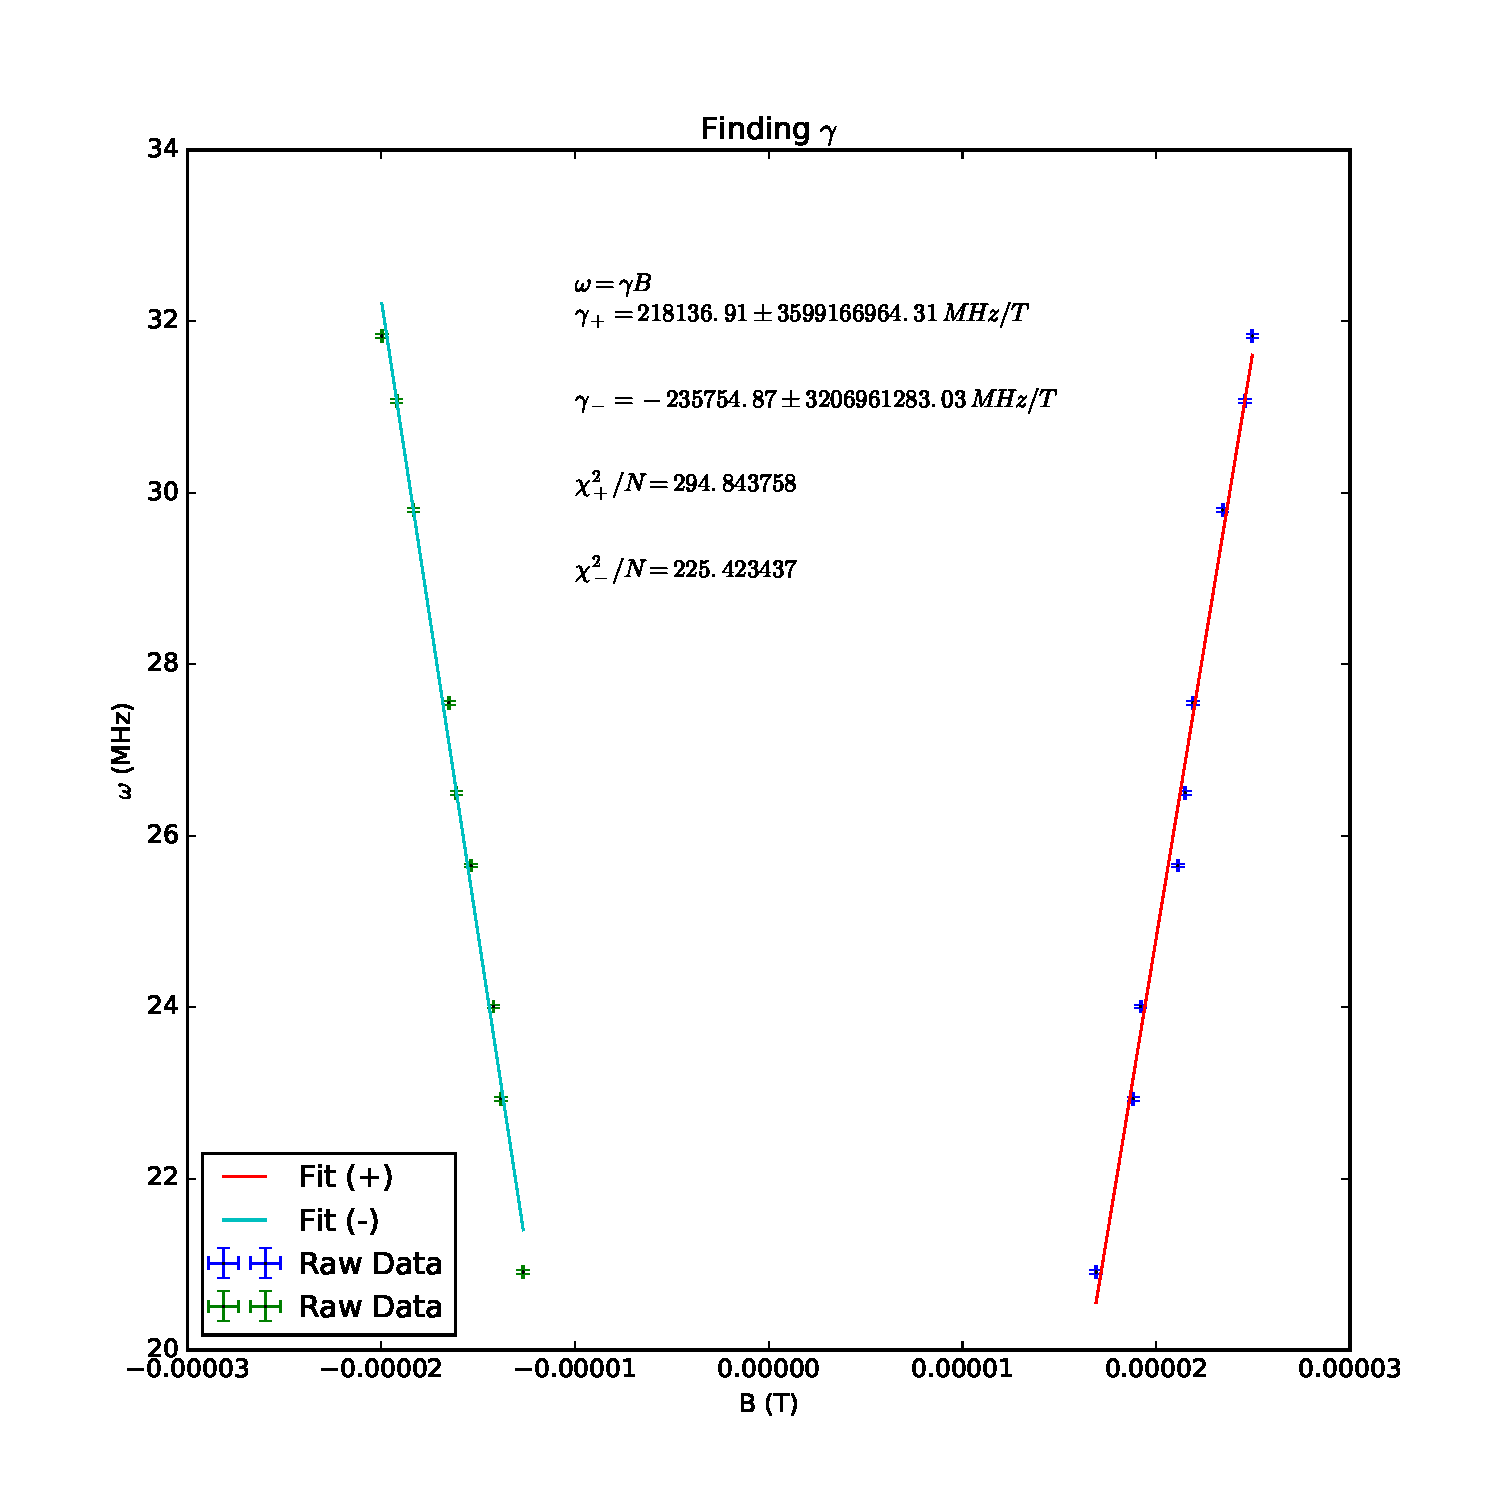
\includegraphics[scale=.5]{../plots/findinggamma.pdf}
		\caption{The sharp-eyed reader will notice that uncertainties on $\gamma_e$ are not shown in the graph.  They are shown in figure 9, for reasons discussed later.}
	\end{figure}

	The reader should notice the alarmingly large values of \redchi, both being over 200.  However, the reader should fear not, for this is due to the alarmingly tiny uncertainties in the measurement.  An illustrative plot is shown in figure 9.  Furthermore, since the amount of data is much larger for this portion of the experiment, I will refrain from tabulating it here.  However, I will demonstrate a calculation showing how we got our uncertainties on the data points.

	\begin{gather*}
		\delta\omega = 0.02 \, M\!H\!z\\
		\frac{\delta V}{V} = \frac{0.8}{V} \, mV\\
		\abs{\vec{B}} = I\times\parens{0.48\times10^{-6}} = V\times\parens{0.48\times10^{-6}} \, T\\
		\delta \vec{B} = \frac{\delta V}{V} \times B
	\end{gather*}
	The uncertainty in $\omega$ comes from variation in the display ($\pm 1$) added to the uncertainty in a digital readout ($\pm$ last digit).  Variation in V comes from our estimates of our ability to get the correct value by maniuplating the oscilloscope readout.  This is likely high, but as figure 9 will show, this is still tiny by comparison to the uncertainty in the fit.

	\begin{figure}[!htb]
		\centering
		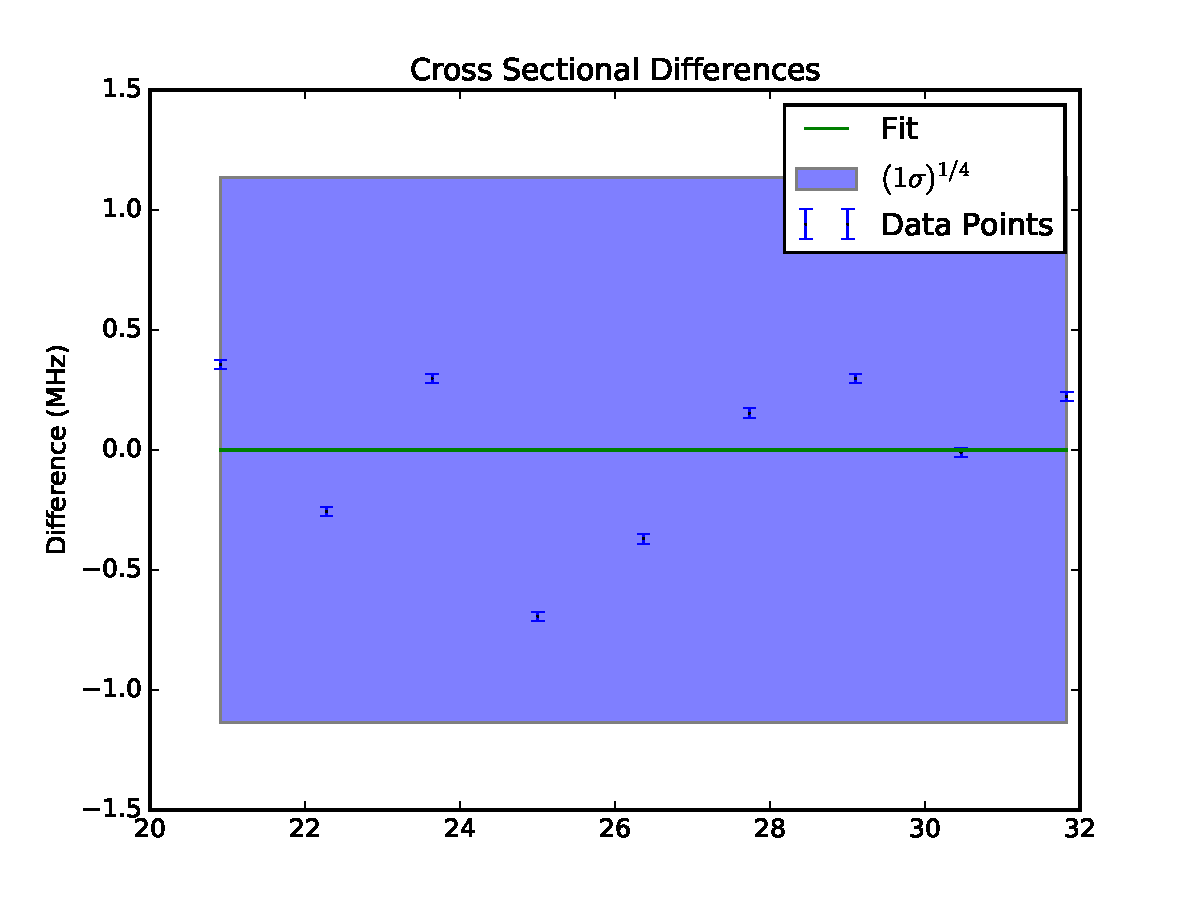
\includegraphics[scale=.5]{../plots/gamma_diff.pdf}
		\caption{The shaded area is $(.05 \times \sigma)^{1/4}$, which comes from massive uncertainties in the fit.  This plot shows the difference between the fit value and the data points.}
	\end{figure}

	We should note that we never actually stated the value for the uncertainty in $\gamma$, and so I will state it here.

	\begin{center}
	\begin{tabular}{|l|l|}
		\hline
		$\gamma_+ \pm \delta\gamma_+$ & $\gamma_- \pm \delta\gamma_-$ \\ 
		\hline
		$\parens*{1.4 \pm 0.7}\times 10^{11}$ & $\parens*{-1.5 \pm 0.5} \times 10^{11}$ \\ 
		\hline
	\end{tabular}
	\end{center}

	It might seem like a mistake that the uncertainty in a fit is so large, given such tiny uncertainties in the data points, but in fact this is because of that.  Since the difference between the points themselves and the fit is large (keep the units in mind, here) and the error is so small, the weighted sum is going to be huge no matter what the fit routine tries.  Due to the large weighted sum, the covariance matrix is going to have huge diagonal elements, at least.  In this case, these are the leading diagonal elements.  Luckily, the off-diagonal (covariance) elements are of order unity, and so the parameters don't covary.  Furthermore, the small offset in the linear fit ($Ax + B$) is of order $B = 1\pm 2$ so this fit truly is $\omega = \gamma B$.  Thus we are stuck with a gigantic variance in the actual value of $\gamma$ that we have calculated.

	\vspace{.25cm}

	Being convinced that something is wrong with our propagation of uncertainty for the measurement of $\omega$ or \B, we checked and rechecked our values and calculations.  We are therefore convinced that there must be an external factor that is causing problems with the fit.  We corrected the uncertainty in the values we measured on the oscilloscope for the current of the Helmholtz coils, in the case that we were much less precise than we thought, which it seems likely that we were.  As can be seen from the plot, which is the version with the corrected uncertainty, we still have huge values.  We also tried to fit the points to higher order polynomials, and attempted to correct the model with various kinds of systematic uncertainty.  None worked.  However, importantly, the model fits quite well, visually.  And even though the standard deviation of the fit is massive, the points lie more or less evenly distributed on either side of the fit line.  Thus we are lead to conclude that our data is not at all going to revolutionalize the study of electron spin resonance, but we have some agreement with the literature values, as shown in the table below.

	\begin{center}
	\begin{tabular}{|l|l|l|}
		\hline
		$\gamma_{exp} \pm \delta\gamma_{exp}$ & $\gamma_{lit}$ & Confidence \\
		\hline
		$(1.4 \pm 0.7) \times 10^{11}$ & $1.76085 \times 10^{11}$ & 57.7\% \\
		$(1.5 \pm 0.5) \times 10^{11}$ & $1.76085 \times 10^{11}$ & 57.4\% \\
		\hline
	\end{tabular}
	\end{center}

	Overall, the uncertainties in the fit may be justified.  Since our agreement with the literature value using these uncertainties is better than 50\% we come to the conclusion that the the uncertainties that come from the fit help save our analysis and ensure that we do not have false confidence in our values due to small uncertainty in data points, and give credit to the values that were generated where credit is perhaps due.

	\vspace{.25cm}

	We also must discuss why this phenomenon doesn't occur at all when the Helmholtz field is angled to be parallel to the RF field.  We can investigate this by transforming the field of the RF oscillator from a linearly polarized photon to a superposition of circularly polarized photons.

	\begin{gather*}
		\vec{B}(t) = 2B_0\cos{\omega t}\,\hat{x}\\
		\vec{B}(t) = B_0\parens{\cos{\omega t}\,\hat{x} + \sin{\omega t}\,\hat{y}} + B_0\parens{\cos{\omega t}\,\hat{x} - \sin{\omega t}\,\hat{y}}
	\end{gather*}
	which, using Maxwell's equations to find \E and $\vec{S}$, gives
	\begin{gather*}
		E = B_0\parens{\cos{\omega t}\,\hat{y} - \sin{\omega t}\,\hat{x}} + B_0\parens{\cos{\omega t}\,\hat{y} + \sin{\omega t}\,\hat{x}}\\
		\vec{S} = \frac{1}{\mu_0}\parens{\vec{E} \times \vec{B}}\\
		\vec{S} = \frac{B_0^2}{\mu_0}\parens{2\cos^2{\omega t}}\,\hat{z}
	\end{gather*}
	From this it is simple to realize why the phenomenon is non-existent when the external field is parallel to the RF field.  Since the poynting vector is in the $\hat{z}$ direction, which is parallel to the Helmholtz field.  When we move the Helmholtz field, the oscillation and power from that field is no longer aligned with this one, and the electrons do not receive the energy required to jump energy levels.  Thus, we see nothing on the oscilloscope because the electrons don't have the energy to actually create a response.

\section{Conclusion}
	From the data and fits performed here, we can begin to think about the classical analogue to the quantum electron, particularly its agreement with the electron's gyromagnetic ratio.  This, we find, is terrible.  We didn't calculate the number of sigma apart the two values are because it is a massive number.  The two values don't agree in the slightest, and that stands to reason.  In general, spinning a billiard ball will not be able to give you a good approximation to the quantum electron.  Furthermore, this approximation is made more problematic by the fact that the electron is, for all intents and purposes, frictionless, while the ball most certainly is not.

	\vspace{.25cm}

	The billiard ball does an excellent job of modeling the quantum electron in that we are able to observe all the phenomena we are interested in.  Because we can see all these reactions happening in a macroscopic system, we will be better able to understand what happens and why in a classical analogue picture.  Of course the electron doesn't slowly change spin, it is either spin up or spin down.  However, it is still a useful tool for visualization.

	\vspace{.25cm}

	Of course, the fundamentals of the physics underlying both parts of the experiment are the same.  The fact that we can describe the ball as a classical system just means that to an excellent approximation it moves like the sum of its parts.  In theory, we could use something much like the quantum system hamiltonian to describe the motion of the whole ball, though it would be quite unweildy.  The convenient part of the classical system is still the macroscopic nature of that portion of the experiment.

	\vspace{.25cm}

	This work was undertaken in cooperation with Ryan Thiermann, and with the help of the TAs and staff of the Advanced Undergraduate Experimental Physics course.  My thanks also to Professor Carlos Wagner, for covering almost exactly the material we needed to properly understand this experiment just before finishing the experiment itself.

\begin{thebibliography}{10}
	\bibitem{DPPH}
		McLauchlan, Keith A, et al. \emph{Electron Paramagnetic Resonance: Volume 17 (Specialist Periodic Reports)}, edited by MJ Davies. Royal Society of Chemistry, 2000.
	\bibitem{lab manual}
		University of Chicago Department of Physics. "Electron Spin Resonance"\\
		https://wiki.uchicago.edu/display/P211manuals/Electron+Spin+Resonance\#ElectronSpinResonance-QUANTUMSYSTEM. (Accessed Oct 23-26, 2015)

	\bibitem{taylor}
		Taylor, John. \emph{An Introduction to Error Analysis}. Sausalito: University Science Books, 1997.

	\bibitem{ceres}
		Agarwal, Sameer and Mierle, Kier, et al. "Ceres Solver"\\
		http://ceres-solver.org. (Accessed Oct 30-31, 2015).
		
\end{thebibliography}

\begin{appendices}
	\section{Fitting Error Analysis} \label{app:Fitting Error Analysis}
	Most of our error calculations came from fitted values, which in turn came from experimental uncertainty in measuring values.  Because of the way that least-squares routines work, the experimental uncertainty is taken into account when calculating the covariance matrix, which is what we use to estimate uncertainty in fitted values.

	\vspace{.25cm}

	The way that least-squares routines calculate the covariance matrix is by making the following assumption
	\begin{equation*}
		y = f(x) + N(0, I)
	\end{equation*}
	which means that $y$ is a function of $x$ plus some normally distributed background noise that depends on the identity, i.e. there is no covariance of terms in $f(x)$.  Then we can make an estimate called the maximum likelihood estimate that is given by
	\begin{equation*}
		x^* = min_x\abs{\abs{f(x)}}^2
	\end{equation*}
	which is simply the solution to the least-squares problem.  Then, given a full column rank Jacobian of $f$ at $x$, we can calculate the covariance matrix by taking
	\begin{equation*}
		C(x^*) = (J(x)^TJ(x))^{-1}.
	\end{equation*}

	If, however, errors are not given by the normally distributed identity covariance, then we must generalize.
	\begin{equation*}
		y = f(x) + N(0, S)
	\end{equation*}
	where S is a positive semi-definite matrix that gives the error in the parameters including the error between parameters.  Then the maximum likelihood problem becomes
	\begin{equation*}
		x^* = min_x f(x)^T S^{-1} f(x)
	\end{equation*}
	and so the covariance matrix becomes
	\begin{equation*}
		C(x^*) = (J(x)^T S^{-1} J(x))^{-1}.
	\end{equation*}

	\vspace{.25cm}

	This simply shows that our method of error propagation, by simply inputting values for error into the fits and then taking the error returned by the fit is indeed valid.  In other cases, such as when calculating $\vec{L}$ from the mass and radius of the ball described in the apparatus section, we use the uncertainty propagation described in the calculation, simply assuming that it would be normally distributed if we make many measurements.  Due in part to the central limit theorem, we do not believe this to be a problematic assumption.  Furthermore, the model fits, so we will use it.
\end{appendices}


\end{document}